\chapter{Computing a best choice recommendation}
\label{sec:6}

\abstract*{To be written.}

\abstract{To be written.}

%.. seealso:: Lecture 7 notes from the MICS Algorithmic Decision Theory course: [ADT-L7].

\section{What site to choose ?}
\label{sec:6.1}

A SME, specialized in printing and copy services, has to move into new offices, and its CEO has gathered seven \textbf{potential office sites} (see Table \ref{tab:6.1}).

\begin{table}[h]
\caption{The potential new office sites}
\label{tab:6.1}       % Give a unique label
\begin{center}
  %\begin{small}
    \begin{tabular}{c|l|l|l}
      \hline\noalign{\smallskip}
      ID & Name & Address & Comment\\
      \noalign{\smallskip}\hline\noalign{\smallskip}
    A &   Ave  &  Avenue de la liberté &  High standing city center\\
    B &   Bon  &  Bonnevoie &             Industrial environment\\
    C &   Ces  &  Cessange &              Residential suburb location\\
    D &   Dom  &  Dommeldange &           Industrial suburb environment\\
    E &   Bel  &  Esch-Belval &           New and ambitious urbanization far from the city\\
    F &   Fen  &  Fentange &              Out in the countryside\\
      G &   Gar  &  Avenue de la Gare &     Main city shopping street\\
      \noalign{\smallskip}\hline
    \end{tabular}
  %\end{small}
\end{center}
\end{table}

Three \textbf{decision objectives} are guiding the CEO's choice:
\begin{enumerate}
\item \emph{minimize} the yearly costs induced by the moving,
\item \emph{maximize} the future turnover of the SME,
\item \emph{maximize} the new working conditions.
\end{enumerate}

The decision consequences to take into account for evaluating the potential new office sites with respect to each of the three objectives are modelled by the following \textbf{coherent family of criteria} Footnote [26].

\begin{table}[h]
\caption{The coherent family of performance criteria}
\label{tab:6.2}       % Give a unique label
\begin{center}
    \begin{tabular}{l|l|l|l}
      \hline\noalign{\smallskip}
      Objective & ID & Name &  Comment\\
      \noalign{\smallskip}\hline\noalign{\smallskip}
    Yearly costs  &       C &   Costs &       Annual rent, charges, and cleaning\\
    \             &  \      & \        &  \ \\
    Future turnover   &   St &   Standing &    Image and presentation\\
    Future turnover   &   V  &  Visibility &  Circulation of potential customers \\
    Future turnover   &   Pr  & Proximity  &  Distance from town center\\
    \                 &   \   & \          &  \  \\
    Working conditions &  W  &  Space   &     Working space\\
    Working conditions &  Cf &  Comfort  &    Quality of office equipment\\
    Working conditions &  P  &  Parking  &    Available parking facilities\\
      \noalign{\smallskip}\hline
    \end{tabular}   
  \end{center}
\end{table}

The evaluation of the seven potential sites on each criterion are gathered in the following \textbf{performance tableau}.

\begin{table}[h]
\caption{Performance evaluations of the potential office sites}
\label{tab:6.3}       % Give a unique label
\begin{center}
    \begin{tabular}{l|c|c|c|c|c|c|c|c}
      \hline\noalign{\smallskip}
    Criterion  &   weight &  A  &      B &       C &       D &       E &        F &        G\\
       \noalign{\smallskip}\hline\noalign{\smallskip}

    Costs     &    45.0  &   35.0K€ &  17.8K€  & 6.7K€  &  14.1K€ &  34.8K€ &  18.6K€ &  12.0K€\\
    \      &        \    &   \      &  \     &   \     &   \    &    \    &    \    &    \ \\
    Proximity     &     32.0  &   100    &  20 &      80    &   70    &   40    &   0    &    60 \\
    Visibility     &     26.0  &   60     &  80  &     70    &   50    &   60    &   0    &    100 \\
    Standing     &     23.0  &   100   &   10   &    0     &   30    &   90    &   70   &    20 \\
    \        &      \    &   \     &   \    &    \     &   \     &   \     &   \    &    \  \\
    Working space     &     10.0  &   75    &   30   &    0     &   55    &   100   &   0    &    50  \\
    Working comfort     &      6.0  &   0     &   100  &    10    &   30    &   60    &   80   &    50 \\
    Parking     &      3.0  &   90    &   30   &    100   &   90    &   70    &   0    &    80 \\
      \noalign{\smallskip}\hline
    \end{tabular}
  \end{center}
\end{table}

Except the \emph{Costs} criterion, all other criteria admit for grading a qualitative satisfaction scale from $0\%$ (worst) to $100\%$ (best). We may thus notice in Table \ref{tab:6.3} that site $A$ is the most expensive, but also $100\%$ satisfying the \emph{Proximity} as well as the  \emph{Standing} criterion. Whereas the site $C$ is the cheapest one; providing however no satisfaction at all on both the \emph{Standing} and the \emph{Working Space} criteria.

In Table \ref{tab:6.3} we may also see that the \emph{Costs} criterion admits the highest significance ($45.0$), followed by the \emph{Future turnover} criteria $(32.0 + 26.0 + 23.0 = 81.0)$, The \emph{Working conditions} criteria are the less significant $(10.0 + 6.0, + 3.0 = 19.0)$. It follows that the CEO considers \emph{maximizing the future turnover} the most important objective ($81.0$), followed by minizing the yearly costs ($45.0$), and less important, \emph{maximizing working conditions} ($19.0$). 

Concerning yearly costs, we suppose that the CEO is indifferent up to a performance difference of $1000.00$€, and he actually prefers a site if there is at least a positive difference of $2500.00$€. The grades observed on the six qualitative criteria (measured in percentages of satisfaction) are very subjective and rather imprecise. The CEO is hence indifferent up to a satisfaction difference of $10\%$, and he claims a significant preference when the satisfaction difference is at least of $20\%$.  Furthermore, a satisfaction difference of $80\%$ represents for him a \emph{considerably large} performance difference, triggering the case given a polarisation of the preferential situations (see [BIS-2013]). 

In view of Table \ref{tab:6.3}, what is now the office site we may recommend to the CEO as \textbf{best choice}?

\section{The \Digraph Performance tableau}
\label{sec:6.2}


A corresponding, \texttt{PerformanceTableau} object, saved in file \texttt{officeChoice.py} is provided in the \texttt{examples} directory of the \Digraph resources. 

We may inspect its actual content with the computing resources provided by the \texttt{perfTabs} module.

\begin{lstlisting}[caption={Inspecting the \texttt{officeChoice} performance tableau},label=list:6.1]
>>> from perfTabs import PerformanceTableau
>>> t = PerformanceTableau('examples/officeChoice')
>>> t
 *------- PerformanceTableau instance description ------*
   Instance class     : PerformanceTableau
   Instance name      : officeChoice
   Actions            : 7
   Objectives         : 3
   Criteria           : 7
   NaN proportion (%) : 0.0
   Attributes         : ['name', 'actions', 'objectives',
                         'criteria', 'weightPreorder',
			 'NA', 'evaluation']
>>> t.showPerformanceTableau()
 *----  performance tableau -----*
  Criteria|  'C'        'Cf'   'P'   'Pr'   'St'   'V'    'W'   
  Weights |  45.00      6.00   3.00  32.00  23.00  26.00  10.00    
  --------|----------------------------------------------------
   'Ave'  | -35000.00   0.00  90.00 100.00 100.00  60.00  75.00  
   'Bon'  | -17800.00 100.00  30.00  20.00  10.00  80.00  30.00  
   'Ces'  |  -6700.00  10.00 100.00  80.00   0.00  70.00   0.00  
   'Dom'  | -14100.00  30.00  90.00  70.00  30.00  50.00  55.00  
   'Bel'  | -34800.00  60.00  70.00  40.00  90.00  60.00 100.00  
   'Fen'  | -18600.00  80.00   0.00   0.00  70.00   0.00   0.00  
   'Gar'  | -12000.00  50.00  80.00  60.00  20.00 100.00  50.00  
\end{lstlisting}

We thus recover all the input data. To measure the actual preference discrimination we observe on each criterion, we may use the \texttt{showCriteria()} method.

\begin{lstlisting}[caption={Inspecting the performance criteria},label=list:6.2]
>>> t.showCriteria(IntegerWeights=True)
 *----  criteria -----*
  C 'Costs'
   Scale = (Decimal('0.00'), Decimal('50000.00'))
   Weight = 45
   Threshold ind : 1000.00 + 0.00x ;  percentile:  9.5
   Threshold pref : 2500.00 + 0.00x ; percentile: 14.3
  Cf 'Comfort'
   Scale = (Decimal('0.00'), Decimal('100.00'))
   Weight = 6
   Threshold ind : 10.00 + 0.00x ;  percentile:   9.5
   Threshold pref : 20.00 + 0.00x ; percentile:  28.6
   Threshold veto : 80.00 + 0.00x ; percentile:  90.5
    ...
\end{lstlisting}

On the \emph{Costs} criterion, $9.5\%$ of the performance differences are considered insignificant and $14.3\%$ below the preference discrimination threshold (see Listing \ref{list:6.2} lines 6-7). On the qualitative \emph{Comfort} criterion, we observe again $9.5\%$ of insignificant performance differences (line 11). Due to the imprecision in the subjective grading, we notice here $28.6\%$ of performance differences below the preference discrimination threshold (Line 12). Furthermore, $100.0 - 90.5 = 9.5\%$ of the performance differences are judged \emph{considerably large} (Line 13); $80\%$ and more of satisfaction differences triggering in fact a polarisation of the preferential situation. Same information is available for all the other criteria. 
 
A colorful comparison of all the performances is shown in Figure \ref{fig:6.1} by the \textbf{heatmap} statistics, illustrating the respective quantile class of each performance. As the set of potential alternatives is tiny, we choose here a classification into performance quintiles.

\begin{lstlisting}
>>> t.showHTMLPerformanceHeatmap(colorLevels=5,\
...                              rankingRule=None)
\end{lstlisting}
    
\begin{figure}[h]
%\sidecaption
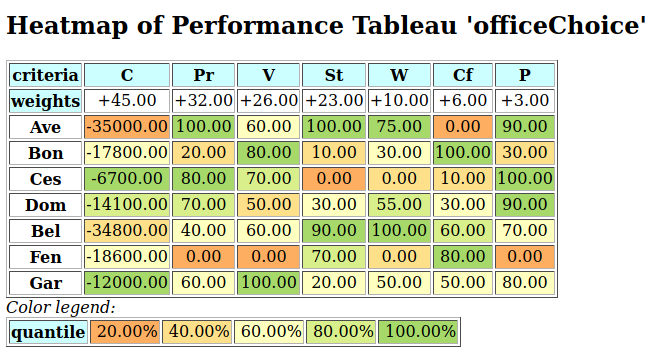
\includegraphics[width=11cm]{Figures/officeChoiceHeatmap.png}
\caption{Unranked heatmap of the office choice performance tableau.}
\label{fig:6.1}       % Give a unique label
\end{figure}

Site $Ave$ shows extreme and contradictory performances: highest \emph{Costs} and no \emph{Working Comfort} on the one hand, and total satisfaction with respect to \emph{Standing}, \emph{Proximity} and \emph{Parking facilities} on the other hand. Similar, but opposite, situation is given for site $Ces$: unsatisfactory \emph{Working Space}, no \emph{Standing} and no \emph{Working Comfort} on the one hand, and lowest \emph{Costs}, best \emph{Proximity} and \emph{Parking facilities} on the other hand. Contrary to these contradictory alternatives, we observe two appealing compromise decision alternatives: sites $Dom$ and $Gar$. Finally, site $Fen$ is clearly the less satisfactory alternative of all.

To help now the CEO choosing the best site, we are going to compute pairwise outrankings (see [BIS-2013]) on the set of potential sites.


\section{Computing the outranking digraph}
\label{sec:6.2}

For two sites $x$ and $y$:
\begin{itemize}
\item $x$ \emph{outranks} $y$, denoted $(x \succsim y)$, is given when there is:
   \begin{enumerate}
     \item A \textbf{majority} of criteria significance concordantly supporting that site $x$ is \emph{at least as satisfactory as} site $y$, and
    \item \textbf{No considerable} counter-performance observed on any discordant criterion.
    \end{enumerate}
\item $x$ \emph{does not outrank} $y$, denoted $(x \not\succsim y)$, is given when there is:
   \begin{enumerate}
    \item A \textbf{majority} of criteria concordantly supporting that site $x$ is \emph{not at least as satisfactory as} site $y$, and
    \item \textbf{No considerable} better performance observed on any discordant criterion.
    \end{enumerate}
\end{itemize}

The credibility of each pairwise outranking situation (see [BIS-2013]), denoted $r(x \succsim y)$, is measured in a bipolar significance valuation $[-1.0, 1.0]$, where \textbf{positive} terms $r(x \succsim y)\, >\, 0.0$ indicate a \textbf{validated}, and \textbf{negative} terms $r(x \succsim y)\, <\, 0.0$ indicate a \textbf{non-validated} outranking situation. The \textbf{median} value $r(x \succsim y)\, = \,0.0$ represents an \textbf{indeterminate} situation (see [BIS-2004a]).   

For computing such a bipolar-valued outranking digraph from the given performance tableau $t$, we use the \texttt{BipolarOutrankingDigraph} constructor from the \texttt{outrankingDigraphs} module. The corresponding \texttt{showHTMLRelationTable} method shows here the resulting bipolar-valued adjacency matrix in a system browser window (see Fig. \ref{fig:6.2}).

\begin{lstlisting}
>>> from outrankingDigraphs import BipolarOutrankingDigraph
>>> g = BipolarOutrankingDigraph(t)
>>> g.showHTMLRelationTable()
\end{lstlisting}

\begin{figure}[h]
\sidecaption
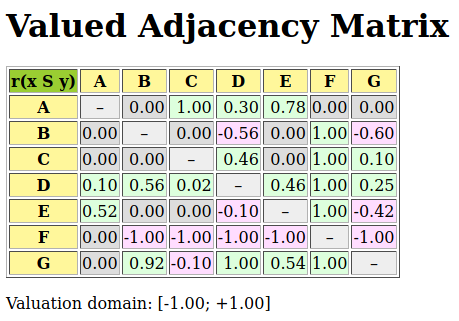
\includegraphics[width=8cm]{Figures/officeChoiceOutranking.png}
\caption{In the resulting outranking relation we may notice that Alternative $D$ is \textbf{positively outranking} all other potential office sites: $D$ is a \Condorcet winner. Yet, alternatives $A$ (the most expensive) and $C$ (the cheapest) are \textbf{not outranked} by any other site; they are in fact \textbf{weak} \Condorcet winners.
}
\label{fig:6.2}       % Give a unique label
\end{figure}

\begin{lstlisting}
>>> g.computeCondorcetWinners()
 ['D']
>>> g.computeWeakCondorcetWinners()
 ['A', 'C', 'D']
\end{lstlisting}

We may get even more insight in the apparent outranking situations when we draw the corresponding \textbf{outranking digraph} (see Fig. \ref{fig:6.2}).

\begin{lstlisting}
>>> g.exportGraphViz('officeChoice')
 *---- exporting a dot file for GraphViz tools ---------*
  Exporting to officeChoice.dot
  dot -Grankdir=BT -Tpng officeChoice.dot -o officeChoice.png
\end{lstlisting}

\begin{figure}[h]
\sidecaption
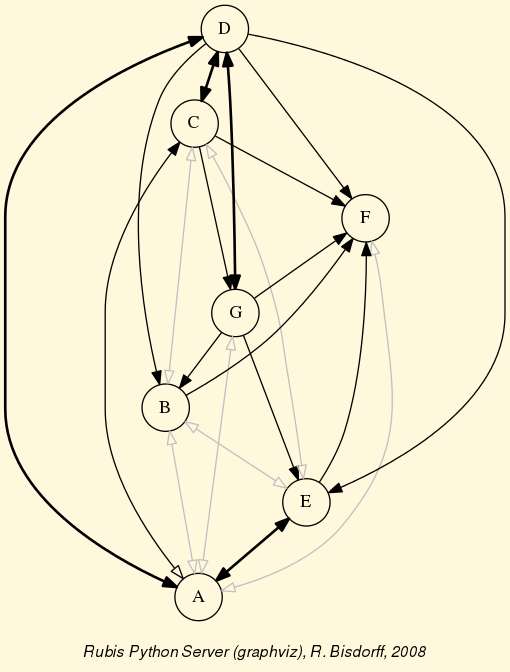
\includegraphics[width=6cm]{Figures/officeChoice.png}
\caption{The office choice outranking digraph.}
\label{fig:6.3}       % Give a unique label
\end{figure}

Outranking digraphs are \emph{weakly complete}, i.e. for all $x$ and $y$ in $X$, $r(x \succsim y)\, <\, 0.0$ implies that $r(y \succsim x)\, \geq\, 0.0$. And, they verify the coduality principle:  $r(x \not\succsim y) \;=\; r(y \succnsim y)$. One may furthermore check that the resulting outranking digraph $g$ here does in fact not admit any cyclic strict preference situation.

\begin{lstlisting}
>>> g.computeChordlessCircuits()
  []
>>> g.showChordlessCircuits()
  No circuits observed in this digraph.
\end{lstlisting}

\section{Computing a \Rubis best choice recommendation}
\label{sec:6.3}

Following the \Rubis outranking method (see [BIS-2008]), potential best choice recommendations are determined by the outranking \textbf{prekernels} --weakly independent and strictly outranking choices-- of the outranking digraph (see the tutorial on computing digraph kernels). The case given, we previously need to break open all chordless odd circuits at their weakest link.

\begin{lstlisting}
>>> from digraphs import BrokenCocsDigraph
>>> bcg = BrokenCocsDigraph(g)
>>> bcg.brokenLinks
  set()
\end{lstlisting}

As we observe indeed no such chordless circuits here, we may directly compute the \textbf{prekernels} of the outranking digraph $g$.

\begin{lstlisting}[caption={Computing outranking and outranked prekernels},label=list:6.3]
>>> g.showPreKernels()
 *--- Computing preKernels ---*
    Dominant preKernels :
    ['D']
       independence :  1.0
       dominance    :  0.02
       absorbency   :  -1.0
       covering     :  1.000
    ['B', 'E', 'C']
       independence :  0.00
       dominance    :  0.10
       absorbency   :  -1.0
       covering     :  0.500
    ['A', 'G']
       independence :  0.00
       dominance    :  0.78
       absorbency   :  0.00
       covering     :  0.700
    Absorbent preKernels :
    ['F', 'A']
       independence :  0.00
       dominance    :  0.00
       absorbency   :  1.0
       covering     :  0.700
    *----- statistics -----
    graph name:  rel_officeChoice.xml
    number of solutions
     dominant kernels :  3
     absorbent kernels:  1
    cardinality frequency distributions
    cardinality     :  [0, 1, 2, 3, 4, 5, 6, 7]
    dominant kernel :  [0, 1, 1, 1, 0, 0, 0, 0]
    absorbent kernel:  [0, 0, 1, 0, 0, 0, 0, 0]
    Execution time  : 0.00018 sec.
    Results in sets: dompreKernels and abspreKernels.
\end{lstlisting}
  
We notice in Listing \ref{list:6.3} three potential best choice recommendations: the \Condorcet winner $D$ (Line 4), the triplet $B$, $C$ and $E$ (Line 9), and finally the pair $A$ and $G$ (Line 14). The best choice recommendation is now given by the \textbf{most determined} prekernel; the one supported by the most significant criteria coalition. This result is shown with the \texttt{showBestChoiceRecommendation} method. Notice that this method actually works by default on the broken chords digraph $bcg$.

\begin{lstlisting}[caption={Computing a best choice recommendation},label=list:6.4]
>>> g.showBestChoiceRecommendation(CoDual=False)
 *****************************************
  Rubis best choice recommendation(s) (BCR)
   (in decreasing order of determinateness)   
   Credibility domain: [-1.00,1.00]
    === >> potential best choice(s)
    * choice              : ['D']
      independence        : 1.00
      dominance           : 0.02
      absorbency          : -1.00
      covering (%)        : 100.00
      determinateness (%) : 51.03
      - most credible action(s) = { 'D': 0.02, }
    === >> potential best choice(s)
    * choice              : ['A', 'G']
      independence        : 0.00
      dominance           : 0.78
      absorbency          : 0.00
      covering (%)        : 70.00
      determinateness (%) : 50.00
      - most credible action(s) = { }
    === >> potential best choice(s)
    * choice              : ['B', 'C', 'E']
      independence        : 0.00
      dominance           : 0.10
      absorbency          : -1.00
      covering (%)        : 50.00
      determinateness (%) : 50.00
      - most credible action(s) = { }
    === >> potential worst choice(s) 
    * choice              : ['A', 'F']
      independence        : 0.00
      dominance           : 0.00
      absorbency          : 1.00
      covered (%)         : 70.00
      determinateness (%) : 50.00
      - most credible action(s) = { }
    Execution time: 0.014 seconds
\end{lstlisting}

We notice in Listing \ref{list:6.4} Line 7 above that the most significantly supported best choice recommendation is indeed the \Condorcet winner $D$ supported by a majority of $51.03\%$ of the criteria significance (see Line 12). Both other potential best choice recommendations, as well as the potential worst choice recommendation, are not positively validated as best, resp. worst choices. They may or may not be considered so. Alternative $A$, with extreme contradictory performances, appears both, in a best and a worst choice recommendation (see Lines 15 and 31) and seams hence not actually comparable to its competitors.

\section{Computing \emph{strict best} choice recommendations}
\label{sec:6.4}

When comparing now the performances of alternatives $D$ and $G$ in a pairwise perspective (see below), we notice that, with the given preference discrimination thresholds, alternative $G$ is actually \textbf{certainly} \emph{at least as good as} alternative $D$:  $r(G \succsim D)\, = \, +145/145\, =\, +1.0$.

\begin{lstlisting}[caption={Inspecting pairwise comparisons},label=list:6.5]
>>> g.showPairwiseComparison('G','D')
 *------------  pairwise comparison ----*
  Comparing actions : ('G', 'D')
  crit.  wght.    g(x)      g(y)    diff.  |   ind     pref    concord 	|
   =====================================================================
   'C'  45.00 -12000.00 -14100.00 +2100.00 | 1000.00 2500.00   +45.00 	| 
   'Cf'  6.00     50.00     30.00   +20.00 |   10.00   20.00    +6.00 	| 
   'P'   3.00     80.00     90.00   -10.00 |   10.00   20.00    +3.00 	| 
   'Pr' 32.00     60.00     70.00   -10.00 |   10.00   20.00   +32.00 	| 
   'St' 23.00     20.00     30.00   -10.00 |   10.00   20.00   +23.00 	| 
   'V'  26.00    100.00     50.00   +50.00 |   10.00   20.00   +26.00 	| 
   'W'  10.00     50.00     55.00    -5.00 |   10.00   20.00   +10.00 	|
   =====================================================================
    Valuation in range: -145.00 to +145.00; global concordance: +145.00
\end{lstlisting}

Yet, we must as well notice that the cheapest alternative $C$ is in fact \textbf{strictly outranking} alternative $G$:  $r(C \succsim G)\, =\, +15/145\, >\, 0.0$, and $r(G \succsim C)\, =\, -15/145 \,<\, 0.0$.

\begin{lstlisting}
>>> g.showPairwiseComparison('C','G')
 *------------  pairwise comparison ----*
  Comparing actions : ('C','G')/('G','C')
  crit. wght.   g(x)     g(y)      diff.  |   ind.   pref. ('C','G')/('G','C')|
   ===========================================================================
   'C'   45.00 -6700.00 -12000.00 +5300.00 | 1000.00 2500.00    +45.00/-45.00 | 
   'Cf'   6.00    10.00     50.00   -40.00 |   10.00   20.00     -6.00/ +6.00 | 
   'P'    3.00   100.00     80.00   +20.00 |   10.00   20.00     +3.00/ -3.00 | 
   'Pr'  32.00    80.00     60.00   +20.00 |   10.00   20.00    +32.00/-32.00 | 
   'St'  23.00     0.00     20.00   -20.00 |   10.00   20.00    -23.00/+23.00 | 
   'V'   26.00    70.00    100.00   -30.00 |   10.00   20.00    -26.00/+26.00 | 
   'W'   10.00     0.00     50.00   -50.00 |   10.00   20.00    -10.00/+10.00 |
   ===========================================================================
    Valuation in range: -145.00 to +145.00; global concordance: +15.00/-15.00
\end{lstlisting}
  
To model these \emph{strict outranking} situations, we may recompute the best choice recommendation on the \textbf{codual}, the converse ($\sim$) of the dual ($-$) Footnote[14], of the outranking digraph instance $g$ (see [BIS-2013]), as follows:

\begin{lstlisting}[caption={Computing the strict best choice recommendation},label=list:6.6]
>>> g.showBestChoiceRecommendation(\
...                   CoDual=True,\
...                   ChoiceVector=True)   
* --- Best and worst choice recommendation(s) ---*
  (in decreasing order of determinateness)   
  Credibility domain: [-1.00,1.00]
    === >> potential best choice(s)
    * choice              : ['A', 'C', 'D']
      independence        : 0.00
      dominance           : 0.10
      absorbency          : 0.00
      covering (%)        : 41.67
      determinateness (%) : 50.59
      - characteristic vector = {
             'D': 0.02, 'G': 0.00, 'C': 0.00,
	     'A': 0.00, 'F': -0.02, 'E': -0.02, 'B': -0.02, }
    === >> potential worst choice(s) 
    * choice              : ['A', 'F']
      independence        : 0.00
      dominance           : -0.52
      absorbency          : 1.00
      covered (%)         : 50.00
      determinateness (%) : 50.00
      - characteristic vector = { 'G': 0.00, 'F': 0.00, 'E': 0.00,
	     'D': 0.00, 'C': 0.00, 'B': 0.00, 'A': 0.00, }
\end{lstlisting}				  

It is interesting to notice in Listing \ref{list:6.6} Line 9 that the \textbf{strict best choice recommendation} consists in the set of weak Condorcet winners: $A$, $C$ and $D$. In the corresponding characteristic vector (see Lines 15-16), representing the bipolar credibility degree with which each alternative may indeed be considered a best choice (see [BIS-2006a], [BIS-2006b]), we find confirmed that alternative $D$ is the only positively validated one, whereas both extreme alternatives - $A$ (the most expensive) and $C$ (the cheapest) - stay in an indeterminate situation. They may be potential best choice candidates besides $D$. Notice furthermore that compromise alternative $G$, while not actually included in any outranking prekernel, shows as well an indeterminate situation with respect to \textbf{being or not being} a potential best choice candidate. 

We may also notice (see Line 16 and Line 19) that both alternatives $A$ and $F$ are reported as certainly strict outranked choices, hence as \textbf{potential worst choice recommendation} . This confirms again the global incomparability status of alternative $A$ (see Fig. \ref{fig:6.3}).

\begin{lstlisting}
>>> gcd = ~(-g) # codual of g
>>> gcd.exportGraphViz(fileName='bestChoiceChoice',\
...                    bestChoice=['A','C','D'],\
...                    worstChoice=['F'])
 *---- exporting a dot file for GraphViz tools ---------*
  Exporting to bestOfficeChoice.dot
  dot -Grankdir=BT -Tpng bestOfficeChoice.dot -o bestOfficeChoice.png
\end{lstlisting}

\begin{figure}[h]
\sidecaption
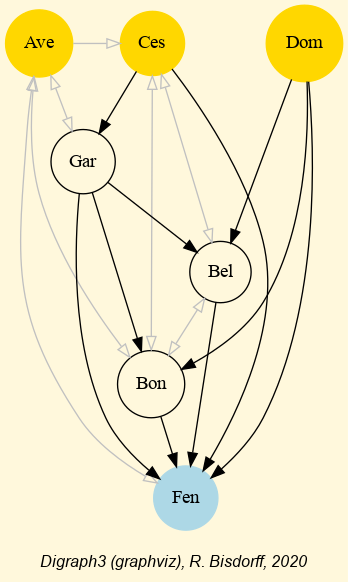
\includegraphics[width=5cm]{Figures/bestOfficeChoice.png}
\caption{Best office choice recommendation from strict outranking digraph.}
\label{fig:6.4}       % Give a unique label
\end{figure}

\section{Weakly ordering the outranking digraph}
\label{sec:6.6}

To get a more complete insight in the overall strict outranking situations, we may use the \texttt{RankingByChoosingDigraph} constructor imported from the \texttt{transitiveDigraphs} module for computing a \textbf{ranking-by-choosing} result from the codual, i.e. the strict outranking digraph instance $gcd$ (see above). If the computing node supports multiple processor cores, best and worst choosing iterations are run in parallel (see Line 3 below).

\begin{lstlisting}
>>> from transitiveDigraphs import RankingByChoosingDigraph
>>> rbc = RankingByChoosingDigraph(gcd)
 Threading ...  # multiprocessing if 2 cores are available
 Exiting computing threads
>>> rbc.showRankingByChoosing()
 Ranking by Choosing and Rejecting
    1st ranked ['D']
       2nd ranked ['C', 'G']
       2nd last ranked ['B', 'C', 'E']
    1st last ranked ['A', 'F']
>>> rbc.exportGraphViz('officeChoiceRanking')
 *---- exporting a dot file for GraphViz tools ---------*
  Exporting to officeChoiceRanking.dot
  dot -Grankdir=TB -Tpng officeChoiceRanking.dot\
                   -o officeChoiceRanking.png
\end{lstlisting}

\begin{figure}[h]
\sidecaption
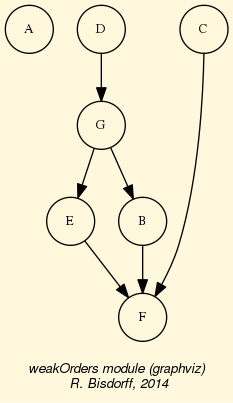
\includegraphics[width=6cm]{Figures/officeChoiceRanking.png}
\caption{In this \textbf{ranking-by-choosing} method, where we operate the \emph{epistemic fusion} of iterated (strict) best and worst choices, compromise alternative $D$ is now ranked before compromise alternative $G$. The overall partial ordering result shows again the important fact that the most expensive site $A$, and the cheapest site $C$, both appear incomparable with most of the other alternatives, as is apparent from the Hasse diagram of the ranking-by-choosing result here.} 
\label{fig:6.5}       % Give a unique label
\end{figure}
	   
The best choice recommendation appears hence depending on the very importance the CEO is attaching to each of the three decision objectives he is considering. In the setting here, where he considers that \emph{maximizing the future turnover} is the most important objective followed by \emph{minimizing the Costs} and, less important, \emph{maximizing the working conditions}, site $D$ represents actually the best compromise. However, if \emph{Costs} do not play much a role, it would be perhaps better to decide to move to the most advantageous site $A$; or if, on the contrary, \emph{Costs} do matter a lot, moving to the cheapest alternative $C$ could definitely represent a more convincing recommendation. 

It might be worth, as an \textbf{exercise}, to modify these criteria significance weights in the \texttt{officeChoice.py} data file in such a way that
\begin{itemize}
\item all criteria under an objective appear \emph{equi-significant}, and
\item all three decision objectives are considered \emph{equally important}.
\end{itemize}

What will become the best choice recommendation under this working hypothesis?  

%.. seealso:: Lecture 7 notes from the MICS Algorithmic Decision Theory course: [ADT-L7].
 
